\documentclass[12pt]{article}
\usepackage{amscd,amssymb,amsthm,amsxtra,exscale,latexsym,verbatim,paralist}
\usepackage{mathrsfs}
\usepackage[T1]{fontenc}
\usepackage{newtxmath,newtxtext}
\usepackage[left = 2cm, top = 2cm, bottom = 2cm, right = 2cm]{geometry}

\usepackage{hyperref}
\usepackage{tikz}
\usetikzlibrary{patterns}

\newcommand{\XB}{\color{black}}
\newcommand{\XBB}{\color{blue}}
\newcommand{\XV}{\color{violet}}
\newcommand{\XR}{\color{red}}
\newcommand{\ds}{\displaystyle}

\setlength{\parindent}{0pt} 
\setlength{\parskip}{\baselineskip}

\theoremstyle{plain}
\newtheorem{ex}{Exercise}

\renewcommand{\proofname}{Solution}

\begin{document}

\title{\textbf{MTH385}: History of Mathematics - Homework \#11}
\date{\today}
\author{\XV\textit{\large{\href{https://github.com/casonk}{Cason Konzer}}}\XB}

\maketitle

\hrulefill

\newpage

%%%%%%%%%%%%%%%%%%%%%%%%%%%%%%%%%%%%%%%%%%%%%%%%%%%%%%%%%%%%%%%%%%%%%%%%%%%%%%%%%%%%%%%%%%%%%%%%%%%%%%%%%%%%%
%%%%%%%%%%%%%%%%%%     #1     %%%%%%%%%%%%%%%%%%%%%%%%%%%%%%%%%%%%%%%%%%%%%%%%%%%%%%%%%%%%%%%%%%%%%%%%%%%%%%%
%%%%%%%%%%%%%%%%%%%%%%%%%%%%%%%%%%%%%%%%%%%%%%%%%%%%%%%%%%%%%%%%%%%%%%%%%%%%%%%%%%%%%%%%%%%%%%%%%%%%%%%%%%%%%

\XBB\hrulefill\XB \\
\begin{ex} [8.2.3]
  Show that the volume of the solid obtained by rotating the portion of $ y = 1/x $ from $ x = 1 $ to $ \infty $ about the $ x $-axis is finite. 
  Show, on the other hand, that its surface area is infinite.
\end{ex}
\XBB\hrulefill\XB \\

\begin{proof}
  \ \\

  \begin{itemize}
    \item $ \ds A = \pi r^{2} \Rightarrow V = \pi \int_{1}^{\infty} (1/x)^{2} \,dx = \pi[-(1/\infty) + (1/1) ]  = \pi  $.
    \item $ \ds C = 2 \pi r \Rightarrow SA = 2 \pi \int_{1}^{\infty} (1/x) \,dx = 2\pi[\ln(\infty) - \ln(1)] = 2\pi\ln(\infty) = \infty $.
  \end{itemize}

\end{proof}

\newpage

Cavalieri's most elegant application of his method of indivisibles was to prove Archimedes' formula for the volume of a sphere. 
His argument is simpler than that of Archimedes, and it goes as follows.

%%%%%%%%%%%%%%%%%%%%%%%%%%%%%%%%%%%%%%%%%%%%%%%%%%%%%%%%%%%%%%%%%%%%%%%%%%%%%%%%%%%%%%%%%%%%%%%%%%%%%%%%%%%%%
%%%%%%%%%%%%%%%%%%     #2     %%%%%%%%%%%%%%%%%%%%%%%%%%%%%%%%%%%%%%%%%%%%%%%%%%%%%%%%%%%%%%%%%%%%%%%%%%%%%%%
%%%%%%%%%%%%%%%%%%%%%%%%%%%%%%%%%%%%%%%%%%%%%%%%%%%%%%%%%%%%%%%%%%%%%%%%%%%%%%%%%%%%%%%%%%%%%%%%%%%%%%%%%%%%%

\XBB\hrulefill\XB \\
\begin{ex} [8.2.4]
  Show that the slice $ z = c $ of the sphere $ x^{2} + y^{2} + z^{2} = 1 $ has the same area as the slice $ z = c $ of the cylinder $ x^{2} + y^{2} = 1 $ outside the cone $ x^{2} + y^{2} = z^{2} $ (Figure~8.2).
\end{ex}
\XBB\hrulefill\XB \\

\begin{center}
  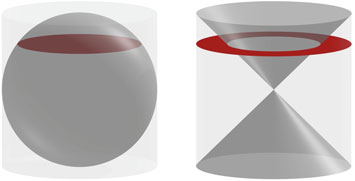
\includegraphics{8_2.jpg}
\end{center}

\begin{proof}
  \ \\

  \begin{itemize}
    \item $ \ds x^{2} + y^{2} = r_{circle}^{2} = 1 - z^{2} \Rightarrow A_{circle} = \pi(1 - z^{2}) $.
    \item $ \ds x^{2} + y^{2} = r_{cylinder}^{2} = 1 \ , \ x^{2} + y^{2} = r_{cone}^{2} = z^{2} \Rightarrow A_{ring} = \pi(r_{cylinder}^{2} - r_{cone}^{2}) = \pi(1 - z^{2}) $.
  \end{itemize}

\end{proof}

\newpage

%%%%%%%%%%%%%%%%%%%%%%%%%%%%%%%%%%%%%%%%%%%%%%%%%%%%%%%%%%%%%%%%%%%%%%%%%%%%%%%%%%%%%%%%%%%%%%%%%%%%%%%%%%%%%
%%%%%%%%%%%%%%%%%%     #3     %%%%%%%%%%%%%%%%%%%%%%%%%%%%%%%%%%%%%%%%%%%%%%%%%%%%%%%%%%%%%%%%%%%%%%%%%%%%%%%
%%%%%%%%%%%%%%%%%%%%%%%%%%%%%%%%%%%%%%%%%%%%%%%%%%%%%%%%%%%%%%%%%%%%%%%%%%%%%%%%%%%%%%%%%%%%%%%%%%%%%%%%%%%%%

\XBB\hrulefill\XB \\
\begin{ex} [8.2.5]
  Deduce from Exercise~8.2.4, and the known volume of the cone, that the volume of the sphere is $ 2 / 3 $ the volume of the circumscribing cylinder.
\end{ex}
\XBB\hrulefill\XB \\

\begin{proof}
  \ \\

  \begin{itemize}
    \item $ \ds V_{cylinder} = 2z \pi r^{2}  $.
    \item $ \ds V_{cone} = z \pi r^{2} / 3 $.
    \item $ \ds V_{sphere} = V_{cylinder} - 2V_{cone} = (6 - 2) z \pi r^{2} / 3 = 4z \pi r^{2} / 3 $.
    \item $ \ds V_{sphere} / V_{cylinder} = (4z \pi r^{2} / 3) / 2z \pi r^{2} = 2 / 3 $.
  \end{itemize}

  Notice in all cases we have $ z = r $ such that we see the common formula $ \ds V_{sphere} = 4 \pi r^{3} / 3 $.
\end{proof}

\newpage

The examples in Exercise~8.3.1 and Exercise~8.3.2 show how tangents can be found by looking for double roots, though it requires some foresight to make the right substitution. With calculus, the process is more mechanical.

%%%%%%%%%%%%%%%%%%%%%%%%%%%%%%%%%%%%%%%%%%%%%%%%%%%%%%%%%%%%%%%%%%%%%%%%%%%%%%%%%%%%%%%%%%%%%%%%%%%%%%%%%%%%%
%%%%%%%%%%%%%%%%%%     #4     %%%%%%%%%%%%%%%%%%%%%%%%%%%%%%%%%%%%%%%%%%%%%%%%%%%%%%%%%%%%%%%%%%%%%%%%%%%%%%%
%%%%%%%%%%%%%%%%%%%%%%%%%%%%%%%%%%%%%%%%%%%%%%%%%%%%%%%%%%%%%%%%%%%%%%%%%%%%%%%%%%%%%%%%%%%%%%%%%%%%%%%%%%%%%

\XBB\hrulefill\XB \\
\begin{ex} [8.3.3]
  Derive the formula of Hudde and Sluse by differentiating $ \sum a_{ij} x^{i} y^{j} = 0 $ with respect to $ x $.
\end{ex}
\XBB\hrulefill\XB \\

\begin{proof}
  \ \\

  \begin{itemize}
    \item $ \ds \frac{d}{dx} \Bigl( \sum a_{ij} x^{i} y^{j} \Bigr) =  \sum \Bigl( a_{ij}i x^{i-1} y^{j} + a_{ij}j x^{i} y^{j-1} \frac{dy}{dx} \Bigr) = 0 $.
    \item $ \ds \sum a_{ij} i x^{i-1} y^{j} = -\sum a_{ij} j x^{i} y^{j-1} \frac{dy}{dx} \Rightarrow \frac{dy}{dx} = -\frac{\ds \sum a_{ij} i x^{i-1} y^{j}}{\ds \sum a_{ij} j x^{i} y^{j-1}}$.
  \end{itemize}

\end{proof}

\newpage

%%%%%%%%%%%%%%%%%%%%%%%%%%%%%%%%%%%%%%%%%%%%%%%%%%%%%%%%%%%%%%%%%%%%%%%%%%%%%%%%%%%%%%%%%%%%%%%%%%%%%%%%%%%%%
%%%%%%%%%%%%%%%%%%     #5     %%%%%%%%%%%%%%%%%%%%%%%%%%%%%%%%%%%%%%%%%%%%%%%%%%%%%%%%%%%%%%%%%%%%%%%%%%%%%%%
%%%%%%%%%%%%%%%%%%%%%%%%%%%%%%%%%%%%%%%%%%%%%%%%%%%%%%%%%%%%%%%%%%%%%%%%%%%%%%%%%%%%%%%%%%%%%%%%%%%%%%%%%%%%%

\XBB\hrulefill\XB \\
\begin{ex} [8.3.4]
  Use differentiation to find the tangent to the folium $ x^{3} + y^{3} = 3axy $ at the point $ (b, c) $.
\end{ex}
\XBB\hrulefill\XB \\

\begin{proof}
  \ \\

  \begin{itemize}
    \item $ \ds 3x^{2} + 3y^{2}\frac{dy}{dx} = 3ay + 3ax\frac{dy}{dx} $.
    \item $ \ds ( y^{2} - ax ) \frac{dy}{dx} = ay - x^{2} $.
    \item $ \ds \frac{dy}{dx} = \frac{ay - x^{2}}{y^{2} - ax} $.
    \item $ \ds \frac{dy}{dx} (b, c) = \frac{ac - b^{2}}{c^{2} - ab} $.
  \end{itemize}


  \begin{center}
    \begin{tikzpicture}
      \draw[] (0,0) -- (-0.25,2.5) -- (0.25,2.5) -- (-0.25,-2.5) -- (0,-7.55) -- (0.25,-2.5) -- (0,0) ;
      \draw[] (0,0) -- (2.5,-0.25) -- (2.5,0.25) -- (-2.5,-0.25) -- (-2.5,0.25) -- (0,0) ;
      \node[blue] () at (0,-0.012222222225) {$\ast$} ;
      \node[blue] () at (0,-7.425) {$\amalg$} ;
      \draw[blue] (1,1) -- (2,2) ;
      \draw[blue] (-1,1) -- (-2,2) ;
      \draw[blue] (-1,-1) -- (-2,-2) ;
      \draw[blue] (1,-1) -- (2,-2) ;
    \end{tikzpicture}
  \end{center}

\end{proof}

\newpage

\end{document}

